% formato FRONTE RETRO
\documentclass[epsfig,a4paper,11pt,titlepage,twoside,openany]{book}
\usepackage{epsfig}
\usepackage{plain}
\usepackage{setspace}
\usepackage[paperheight=29.7cm,paperwidth=21cm,outer=1.5cm,inner=2.5cm,top=2cm,bottom=2cm]{geometry} % per definizione layout
\usepackage{titlesec} % per formato custom dei titoli dei capitoli
\usepackage{graphicx}
\graphicspath{{./images/}}
\usepackage{listings}
\usepackage{xcolor}
\usepackage{glossaries}
\usepackage{hyperref}
\usepackage{wrapfig}
\usepackage[shortlabels]{enumitem}

\definecolor{codegreen}{rgb}{0,0.6,0}
\definecolor{codegray}{rgb}{0.5,0.5,0.5}
\definecolor{codepurple}{rgb}{0.58,0,0.82}
\definecolor{backcolour}{rgb}{0.95,0.95,0.92}

\lstdefinestyle{mystyle}{
    backgroundcolor=\color{backcolour},   
    commentstyle=\color{codegreen},
    keywordstyle=\color{magenta},
    numberstyle=\tiny\color{codegray},
    stringstyle=\color{codepurple},
    basicstyle=\ttfamily\footnotesize,
    breakatwhitespace=false,         
    breaklines=true,                 
    captionpos=b,                    
    keepspaces=true,                 
    numbers=left,                    
    numbersep=5pt,                  
    showspaces=false,                
    showstringspaces=false,
    showtabs=false,                  
    tabsize=2
}

\lstset{style=mystyle}

% JSON highlight definition
\definecolor{delim}{RGB}{20,105,176}
\definecolor{numb}{RGB}{106, 109, 32}
\definecolor{string}{rgb}{0.64,0.08,0.08}
\lstdefinelanguage{json}{
    numbers=left,
    numberstyle=\small,
    rulecolor=\color{black},
    showspaces=false,
    showtabs=false,
    breaklines=true,
    postbreak=\raisebox{0ex}[0ex][0ex]{\ensuremath{\color{gray}\hookrightarrow\space}},
    breakatwhitespace=true,
    basicstyle=\ttfamily\small,
    upquote=true,
    morestring=[b]",
    stringstyle=\color{string},
    literate=
     *{0}{{{\color{numb}0}}}{1}
      {1}{{{\color{numb}1}}}{1}
      {2}{{{\color{numb}2}}}{1}
      {3}{{{\color{numb}3}}}{1}
      {4}{{{\color{numb}4}}}{1}
      {5}{{{\color{numb}5}}}{1}
      {6}{{{\color{numb}6}}}{1}
      {7}{{{\color{numb}7}}}{1}
      {8}{{{\color{numb}8}}}{1}
      {9}{{{\color{numb}9}}}{1}
      {\{}{{{\color{delim}{\{}}}}{1}
      {\}}{{{\color{delim}{\}}}}}{1}
      {[}{{{\color{delim}{[}}}}{1}
      {]}{{{\color{delim}{]}}}}{1},
}

\newglossarystyle{mystyle}{
    \glossarystyle{long}
    \renewenvironment{theglossary}
        {\begin{longtable}{p{3cm}p{\glsdescwidth}}}
        {\end{longtable}}
}

% supporto lettere accentate
%\usepackage[latin1]{inputenc} % per Windows;
\usepackage[utf8x]{inputenc} % per Linux (richiede il pacchetto unicode);
%\usepackage[applemac]{inputenc} % per Mac. 

\singlespacing

\usepackage[english]{babel}

% To compile the glossary do "makeindex -s Bitussi_Matteo_Informatica_21.ist  -o Bitussi_Matteo_Informatica_21.gls Bitussi_Matteo_Informatica_21.glo"

\newglossaryentry{SAML}
{
    name=SAML,
    description={Security Assertion Markup Language, is an SSO protocol}
}
\newglossaryentry{OIDC}
{
    name=OIDC,
    description={Open ID Connect, is a SSO protocol} 
}
\newglossaryentry{OAuth}
{
    name=OAuth,
    description={OAuth, is a SSO protocol}
}
\newglossaryentry{session track}
{
    name=session track,
    description={The list of action the browser is told to do}
}

\makeglossaries

\begin{document}

% nessuna numerazione
\pagenumbering{gobble}
\pagestyle{plain}

\thispagestyle{empty}

\begin{center}
  \begin{figure}[h!]
    \centerline{
\psfig{file=marchio_unitrento_colore_it_202002.eps,width=0.6\textwidth}}
  \end{figure}

  \vspace{2 cm} 

  \LARGE{Dipartimento di Ingegneria e Scienza dell’Informazione \\ Departement of Information Engineering and Computer Science \\}

  \vspace{1 cm} 
  \Large{Bachelor's Degree in \\ Computer Science}

  \vspace{2 cm} 
  \Large\textsc{Final dissertation\\} 
  \vspace{1 cm} 
  \Huge\textsc{Declarative Specification of Pentesting Strategies for Browser-based Security Protocols:
  the Case Studies of SAML and OAuth/OIDC\\}
  %\Large{\it{Implementation of an automatic testing language and tool to test HTTP browser based protocols}}


  \vspace{1 cm} 
  \begin{tabular*}{\textwidth}{ c @{\extracolsep{\fill}} c }
  \Large{Supervisor} & \Large{Student}\\
  \Large{Silvio Ranise}& \Large{Matteo Bitussi}\\
  \end{tabular*}

  \vspace{0.5 cm} 
  \begin{tabular*}{\textwidth}{ c @{\extracolsep{\fill}} c }
  \Large{Co-Supervisors} & \Large{}\\
  \Large{Andrea Bisegna}& \Large{}\\
  \Large{Roberto Carbone}& \Large{}\\
  \end{tabular*}

  \vspace{2 cm} 

  \Large{Academic year 2021/2022}
  
\end{center}



\clearpage

% Ringraziamenti
\thispagestyle{empty}

\begin{center}
  {\bf \Huge Ringraziamenti}
\end{center}

\vspace{4cm}


\emph{
  ...thanks to... TODO (in italiano)
}

\clearpage
\pagestyle{plain} % nessuna intestazione e pie pagina con numero al centro


% inizio numerazione pagine in numeri arabi
\mainmatter

%%%%%%%%%%%%%%%%%%%%%%%%%%%%%%%%%%%%%%%%%%%%%%%%%%%%%%%%%%%%%%%%%%%%%%%%%%
%%%%%%%%%%%%%%%%%%%%%%%%%%%%%%%%%%%%%%%%%%%%%%%%%%%%%%%%%%%%%%%%%%%%%%%%%%
%% Nota
%%%%%%%%%%%%%%%%%%%%%%%%%%%%%%%%%%%%%%%%%%%%%%%%%%%%%%%%%%%%%%%%%%%%%%%%%%
%% Si ricorda che il numero massimo di facciate e' 30.
%% Nel conteggio delle facciate sono incluse 
%%   indice
%%   sommario
%%   capitoli
%% Dal conteggio delle facciate sono escluse
%%   frontespizio
%%   ringraziamenti
%%   allegati    
%%%%%%%%%%%%%%%%%%%%%%%%%%%%%%%%%%%%%%%%%%%%%%%%%%%%%%%%%%%%%%%%%%%%%%%%%%
%%%%%%%%%%%%%%%%%%%%%%%%%%%%%%%%%%%%%%%%%%%%%%%%%%%%%%%%%%%%%%%%%%%%%%%%%%

% indice
\tableofcontents
\clearpage

\chapter*{Abstract} % senza numerazione

\addcontentsline{toc}{chapter}{Abstract} % da aggiungere comunque all'indice
% L'abstract deve essere un riassunto dell'introduzione, contesto, motivazione, contributi
This thesis deals with the work started in my internship at Fondazione Bruno Kessler (FBK) in the context of browser-based protocols (based on HTTP) security testing.
In the last years, there has been a constantly rising number of services transitioning from physical to virtual, such as health care and government services, also due to the Covid-19 pandemics. This was done to simplify some procedures and make them faster to be accomplished. However, some security and privacy concerns arise from this transition. A high quantity of sensitive data could be at risk of unwanted access. Software and security engineers have to implement the service's software and manage the data that the software is working with. They will rely on browser-based security protocols to ensure that security requirements such as user identity, the connection between the service and the user, and the integrity of data are met. 

To ensure that all these security requirements are respected during the implementation of the service, there is the need to test the implemented services against the well-known vulnerabilities of the protocols used. Usually, to do that, a software engineer or a security tester, which will be called tester below, will act like an attacker trying to see, edit, and deny access to the data in the services. The tester will use a software to intercept the HTTP messages (from now on messages) between the service and the tester's browser. It will be possible for the tester to edit or remove the messages, simulate an attack, and see if the service is vulnerable. The tester will have to gather all the well-known vulnerabilities related to the used protocols and test them manually. The pentesting is time-consuming and could be done improperly if the tester is not qualified to do it. A software is needed to automatically test the services against the well-known vulnerabilities, which could give a result of whether the services are vulnerable.

The work in this thesis is about the design and implementation of the automatic HTTP pentesting software (from now on tool) and its relative declarative specification language. The tool addresses the challenges highlighted above, such as the automation of the pentesting phase to improve its precision and the design of a language for the specification of the tests. Other software has been evaluated before the start of this work, some of them missed the automation part, others were limited in terms of the possible security tests (from now on tests) to be done. For these reasons, a tool and language have been designed and implemented. First, a declarative specification of pentesting strategies has been designed, simultaneously with the design of an approach to execute the pentesting strategies. Next, the implementation of a tool to execute the pentesting strategies has been done. To test the correctness of the implemented tool and the expressiveness of the proposed specification language, a test definition for \gls{OAuth}/OIDC, a web security protocol, has been written in the implemented language and used during development.

The implemented tool and language have proved to be working in two different use cases, with OAuth/OIDC and SAML. The results obtained by the tool have also been confirmed by comparison with the results of similar software; they have proved to be correct. Lastly, the objectives fixed at the beginning of the work were accomplished, the software and language created are valuable tools to help the tester discover vulnerabilities in services. The definition of an OAuth/OIDC and SAML test suite covering the well-known vulnerabilities is useful as the tester does not need to write them every time to test them. Depending on the service to test, what has to be changed are the automation actions to be executed during testing, as the web pages may be different, so the actions to be accomplished have to be different. Future work has been planned to extend the tool with other functionalities and support other protocols. 







\clearpage

% gruppo per definizone di successione capitoli senza interruzione di pagina
\begingroup
% nessuna interruzione di pagina tra capitoli
% ridefinizione dei comandi di clear page
\renewcommand{\cleardoublepage}{}
%\renewcommand{\clearpage}{}
% redefinizione del formato del titolo del capitolo
% da formato
%   Capitolo X
%   Titolo capitolo
% a formato
%   X   Titolo capitolo 

\titleformat{\chapter}
{\normalfont\Huge\bfseries}{\thechapter}{1em}{}

\titlespacing*{\chapter}{0pt}{0.59in}{0.02in}
\titlespacing*{\section}{0pt}{0.20in}{0.02in}
\titlespacing*{\subsection}{0pt}{0.10in}{0.02in}

%%%%%%%%%%%%%%%%%%%%%%%%%%%%%%%%
% lista dei capitoli
%
% \input oppure \include
%
\printglossary[style=mystyle]
\chapter{Introduction}
\label{chap:introduction}
In the last years, we are seeing a constant transition from physical to virtual, this is the case of bank transactions, government documents, health care data, and almost anything that can be virtualized. This is a great step forward, the storage is optimized and more easily accessible, facilitating the cataloging of the documents. But there are also some big concerns about security of that data, as it is virtual, the access to it is regulated by some authentication protocols instead of a physical identification of the subject accessing the physical documents. This means that it has to be checked whether the person accessing the data is the one that is claiming to be. The three basic principles over which data security is based are confidentiality, integrity and availability of data, this principle is called the CIA triad \cite{cia_triad}.
If those requirements are not met, sensitive data could be made inaccessible or even at risk of access from unauthorized parties, as a result, critical services for health care could be inaccessible, this is what happened for example in Lazio \cite{lazio_hacker_0,lazio_hacker_1}, Italy, on August 2021, where, because of a RansomWare infecting the internal computer network of the region, and keeping it down for multiple days, the covid vaccines and other health-care services could not be booked. Moreover, a lot of data in the systems has been encrypted, and so, denied of any access. It has to be said that preventing RansomWares infections is not the aim of this thesis, but this is a good example of what the consequences of exploiting a vulnerability could be. 

In this thesis the considered services are web-services (from now on service) that rely on browser-based HTTP security protocols. Browser-based protocols are the one used to secure web services communications and . The developing has been done with a particular focus over Identity Management (IdM) protocols such as Security Assertion Markup Language and OAuth, but, without limiting the possible applications to these protocols.
To ensure that the CIA triad requirements are satisfied, there is a need to test all the implementations of the protocols used by the service, that are liable of the security of the data. The services that provide access to the data has to be designed properly and tested by a software engineer or a security tester (from now on tester), over the well-known vulnerabilities. The well-known vulnerabilities are vulnerabilities of the protocols that have been discovered over time, and that are known to exist, the service should be built in a way to avoid them, and should be tested over them. But, there could arise some problems, for instance, the tester should be qualified to test the protocols and should know how they work, this is not always the case, as software engineers are sometimes responsible for doing that. Another problem is that due to the fast-evolving nature of protocols, new vulnerabilities will eventually be found, and so, new tests will have to be defined or old tests would have to be edited. This is a lot of work to be done by the tester. The result is that some vulnerabilities could remain undiscovered, representing a weakness in the system. The work of this thesis propose a new automated testing software and a language to help the tester to test the web-protocols used in the services mentioned above. 

Some softwares to test specific protocols and vulnerabilities already exist \cite{wendy_barreto,claudio_grisenti}, but they are usually very specific and hardcoded in a way that the tests could not be easily edited by the tester. Other tools exist, but they are not usually automated. With this work, I wanted to create a software that could be used to test any type of browser-based HTTP protocol and that could specify the tests in an abstract way, allowing the editing and adding. In order to do this, a new language will be used to specify the tests, and a software will be implemented to execute them. The test results will be evaluated by an oracle, that is composed by a series of components that are responsible for telling if the test is passed or not.

In this thesis the design and implementation of this new software will be discussed.

\section{Contributions}
The contributions of this thesis are the following:
\begin{itemize}
    \item A language to specify tests for browser-based HTTP protocols, that makes possible to customly specify the tests based on the user needs
    \item A methodology to execute the tests specified by the language
    \item Implementation of a dedicated tool to execute the tests defined by the language
    \item An use-case scenario of an IdM protocol
    \item Experimental analysis and a test specification of OAuth/OIDC protocol
\end{itemize}

\section{Structure of the thesis}
The thesis is structured as follows:
\begin{itemize}
    \item \textbf{Chapter \ref{chap:Background}, Background}: A brief introduction over the concepts and softwares used in the rest of the thesis
    \item \textbf{Chapter \ref{chap:Design}, Design of the testing language}: The design of the tool and the testing language
    \item \textbf{Chapter \ref{chap:Implementation}, Implementation}: The implementation of the tool and the testing language
    \item \textbf{Chapter \ref{chap:Use_cases}, Use cases}: Use cases of the work of this thesis
    \item \textbf{Chapter \ref{chap:Related_work}, Related work}: Other works related to this
    \item \textbf{Chapter \ref{chap:Conclusions}, Conclusions and future works}: Conclusions, results, and works that could be done in the future
\end{itemize}





\clearpage 
\printglossary

\chapter{Background}
In this chapter the subjects needed to comprehend the rest of the thesis will be discussed. The most common subjects will be ignored, giving a focus on the more specific and less common ones.

\section{Burp Suite community edition}
Burp Suite Community Edition (from now on \Gls{burp}) is one of the most used application security testing software for web security testing. It works by the use of a proxy server over which a browser redirects the traffic to. The proxy does like a Man In The Middle attack, taking the input traffic from the browser and replying the messages to the target service, giving also transparency over the TSL or SSL encryption. \Gls{burp} has access to the proxy, it can sniff HTTP packets and can edit them before they are forwarded to the browser or the target service. \Gls{burp} also gives the possibility of creating custom plugins giving to the developers access to the java API. This is exactly how the tool will be implemented, using \Gls{burp} as a base over which develop the software that will be executing the tests. The plugin (from now on tool) will be able to intercept, read and edit messages that pass through the \Gls{burp}'s proxy by the use of \Gls{burp}'s API.

\section{Regex}
Regex stands for regular expression, it's a sequence of symbols that define an ensemble of strings that can be matched by it. There is a list of symbols that can be used to specify what characters to match. For example if we want to find the value of the "Host" header in an HTTP message, we want to define a regex like this one: \verb|Host:\s?.*|
This regex will search for the string "Host:" followed by 0 or 1 whitespace, and all the characters that follows until "\verb|\n|" has found. This is a complete explanation of the symbols used in this example:
\begin{itemize}
    \item \verb|\s| is the whitespace character
    \item \textbf{?} is an operator that tells that the preceding symbol will be matched 0 or 1 times
    \item \textbf{*} is an operator that tells that the preceding symbol will be matched 0 or more times
    \item \textbf{.} matches any character except line breaks
\end{itemize}

\section{IdM protocols: SAML and OAuth}
The so-called IdM protocols are protocols that deals with identity management. For the scope of this thesis, SAML and \Gls{OAuth} 2.0 (from now on \Gls{OAuth}) will be discussed, as they are used in the examples and in the related works.

Both \Gls{SAML} and \Gls{OAuth} are Single Sign-On (SSO) protocols, they follow an authentication scheme that allows a user to log in with a single ID and password to any of several related, yet independent, software systems, a more complete explanation can be found in \cite{claudio_grisenti}. 
The difference between \Gls{SAML} (Security Assertion Markup Language) and \Gls{OAuth} is how they work, but their objective is the same, to certificate the identity of a given person in different circumstances.

\subsection{OAuth}
As stated in \cite{ietf_oauth2}, The \Gls{OAuth} authorization framework enables a third-party application to obtain limited access to an HTTP service, either on behalf of a resource owner by orchestrating an approval interaction between the resource owner and the HTTP service, or by allowing the third-party application to obtain access on its own behalf.
A series of messages has to be exchanged between the two parties in order to authenticate a resource owner that wants to access some reserved data in a service.

\subsection{SAML - Security Assertion Markup Language}
As stated in \cite{ietf_SAML}, "The Security Assertion Markup Language (\Gls{SAML}) 2.0 is an XML-based framework that allows identity and security information to be shared across security domains. The Assertion, an XML security token, is a fundamental construct of \Gls{SAML} that is often adopted for use in other protocols and specifications. An Assertion is generally issued by an Identity Provider and consumed by a Service Provider that relies on its content to identify the Assertion's subject for security-related purposes."






\clearpage
\chapter{Design}

\section{The Language}
The idea was to think of a language that could implement all the possible actions which a security tester would be wanting to do on a multipart webapp test.\\
I had to decide how to write and define the actual tests, i thought i could define a proper language with a dedicated parser, but it was not worth the effort, as there are already some well-tested alternatives available. I found a great alternative: i used JSON as a base over which write the tests. It is a convinient way of defining gerarchical sturctures like tests could be.
The gerarchical structure and the details of the language will be discussed in the next charapter.

\subsection{Language structure}
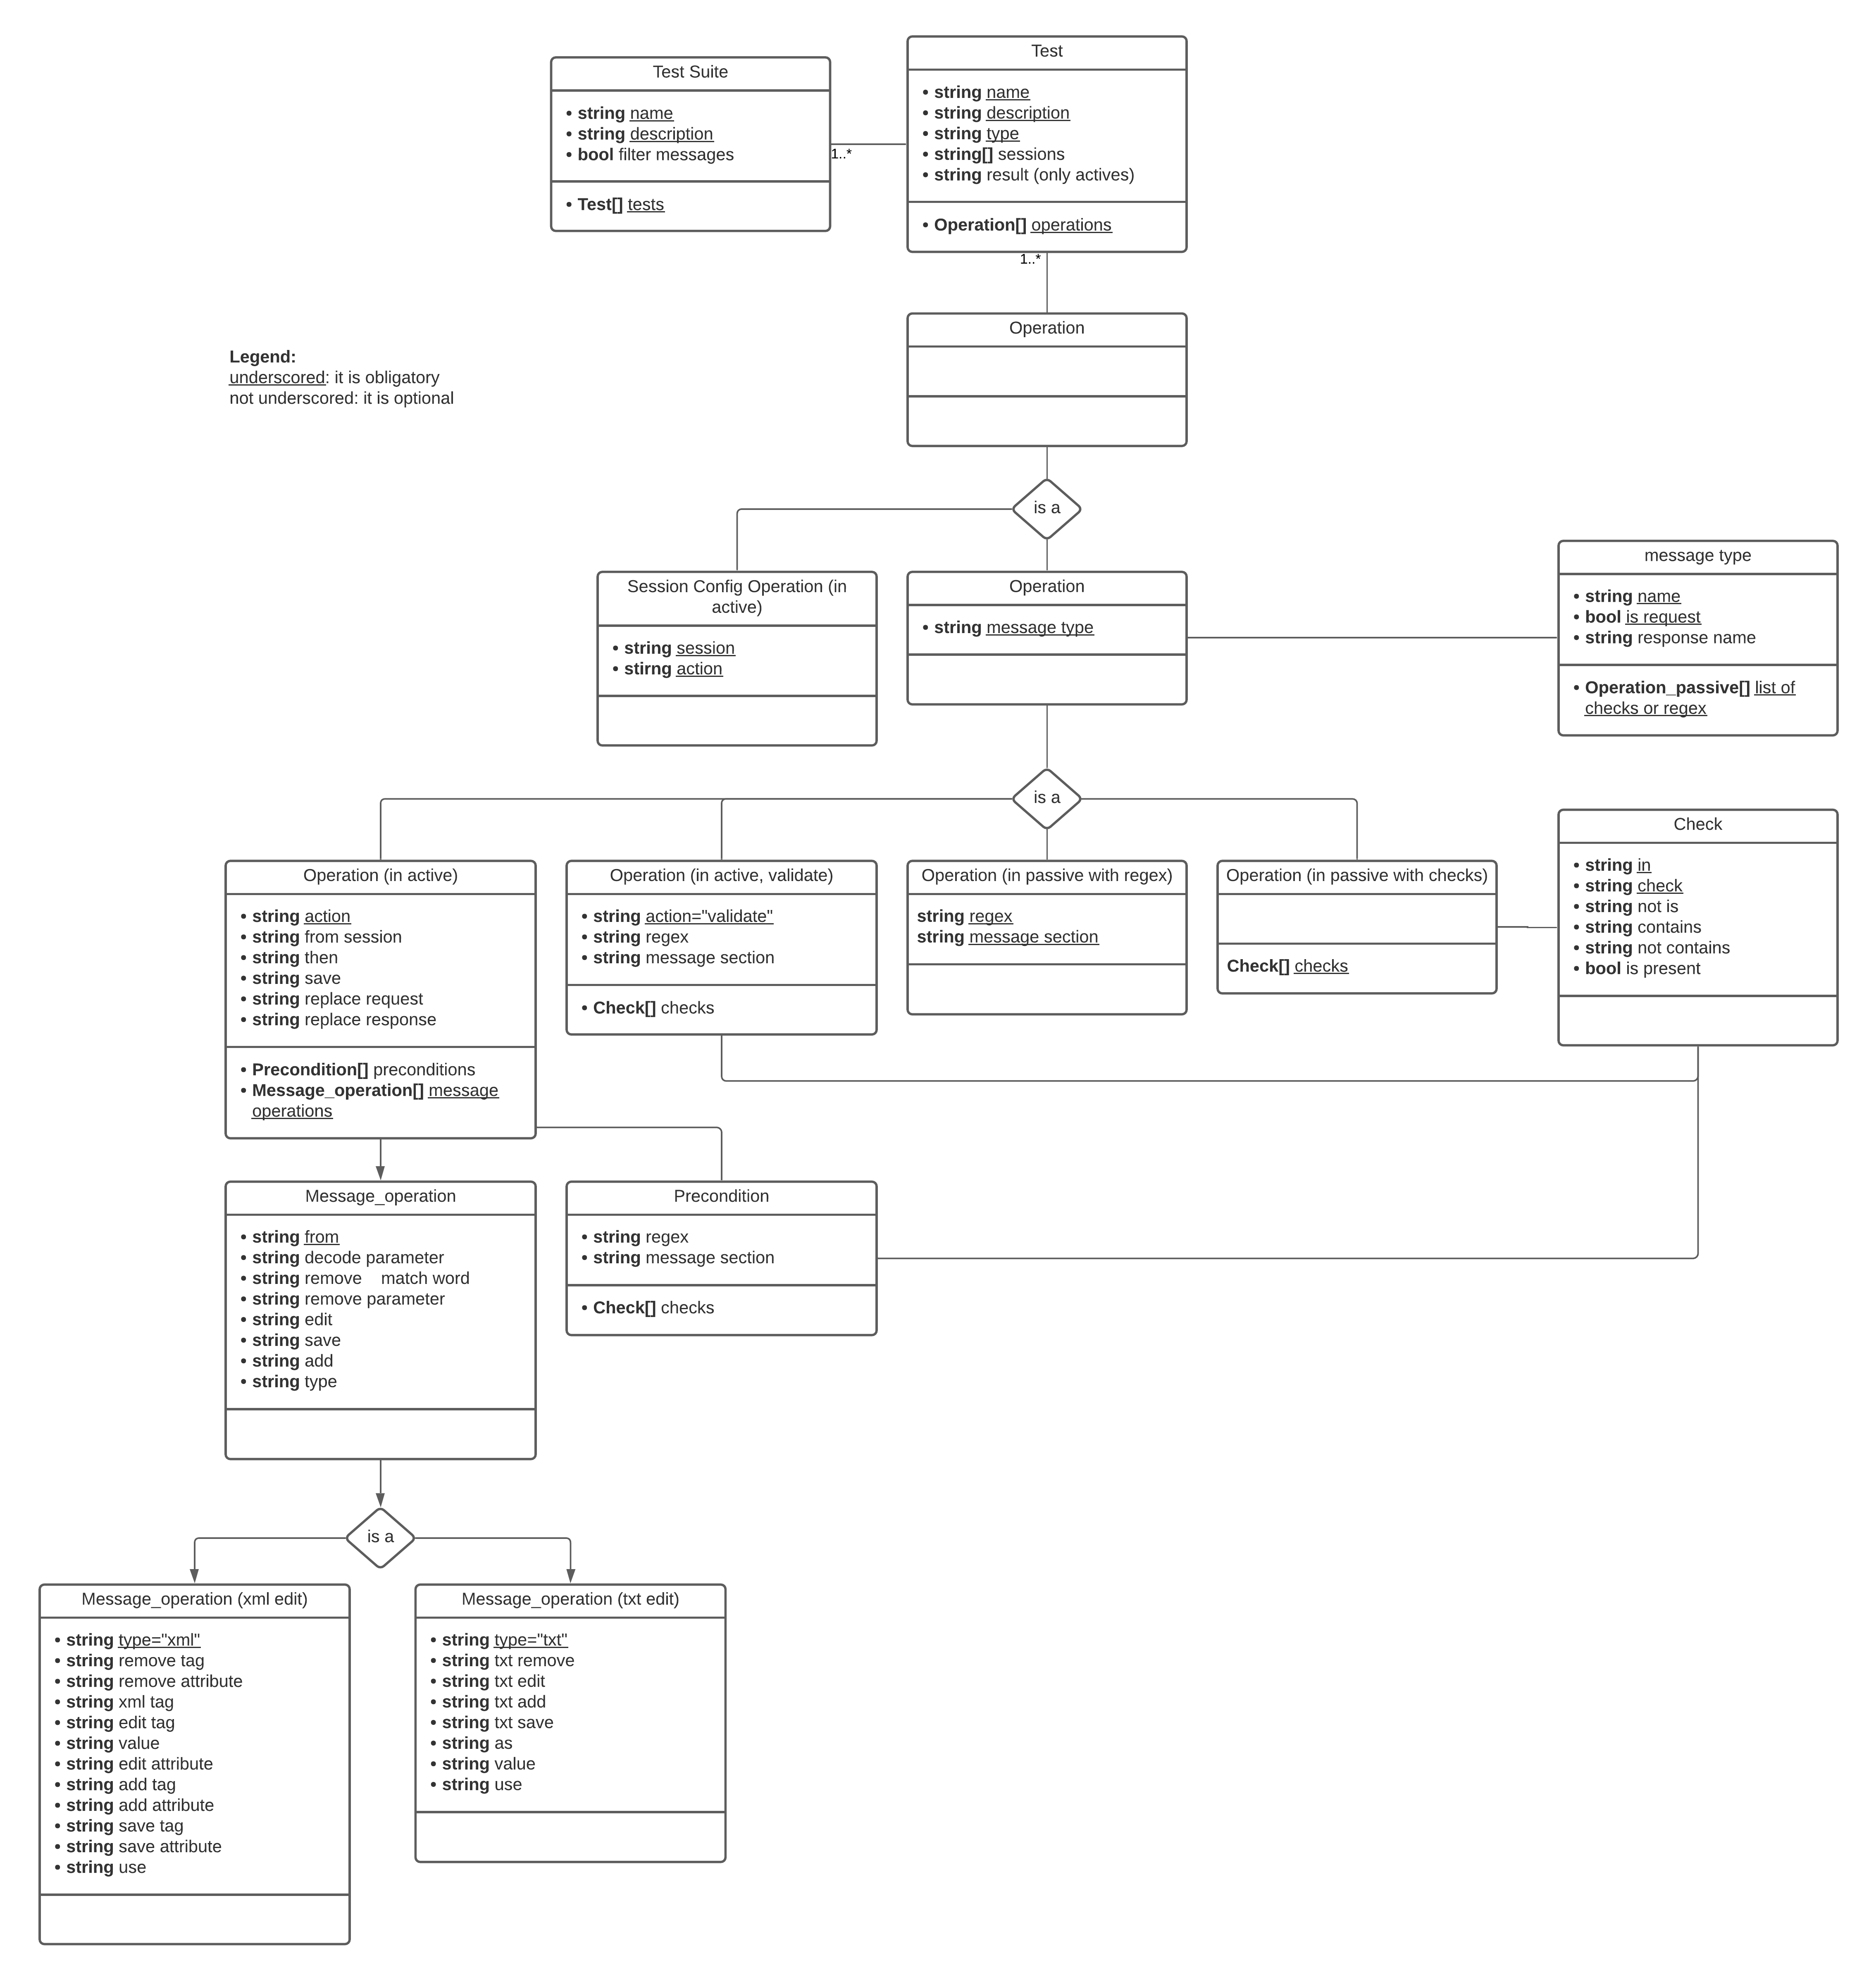
\includegraphics[width=\textwidth]{language_structure.png}

\subsubsection{Test suite}
The test suite is the main component which contains all the other one, it is composed by:
\begin{itemize}
    \item Test suite name, the name of the test suite
    \item Test suite description, the description of the test suite
    \item Tests, which is a list containing the tests to be executed
\end{itemize}

\subsubsection{Test}
The Test object is the one that actually defines a test. As said earlier, a test is contained in a Test Suite, and has various items:
\begin{itemize}
    \item name
    \item description
    \item type, it can be "active" or "passive"
    \item sessions, which is a list of the sessions which are needed in this test
    \item result, (only for actives) it defines the conditions over which the test is considered passed or not.
    \item operations, a list of operation objects which will be executed in the Test object
\end{itemize}

it can be defined either as an active or a passive test, depending on the type of actions it has to do on the intercepted messages. If a doesn't need to manipulate the flow or the content of the messages, then it is considered passive, otherwise it is considered active.
The list of operations is executed iteratively one after the other.

\subsubsection{Operation}
The operation object is the thing that define what a test actually does. As shown in the image above, an operation could be either a standard operation or a session config operation, the latter is used to manage the sessions for the active tests (i.e. start, stop, pause). Depending on the type of test which an Operation is defined into, the standard Operation can be active or passive.
\\A \textbf{passive} operation should contain one of the following options:
\begin{itemize}
    \item A list of Check objects
    \item A regex inspection
\end{itemize}
A regex operaton executes an inspection in


\section{The oracle}



\clearpage
\chapter{Implementation of the tool}
\label{chap:Implementation}
This chapter will discuss the implementation of the language and the tool, the problems faced, and the adopted solutions.

\section{General overview of the tool}
\begin{figure}
    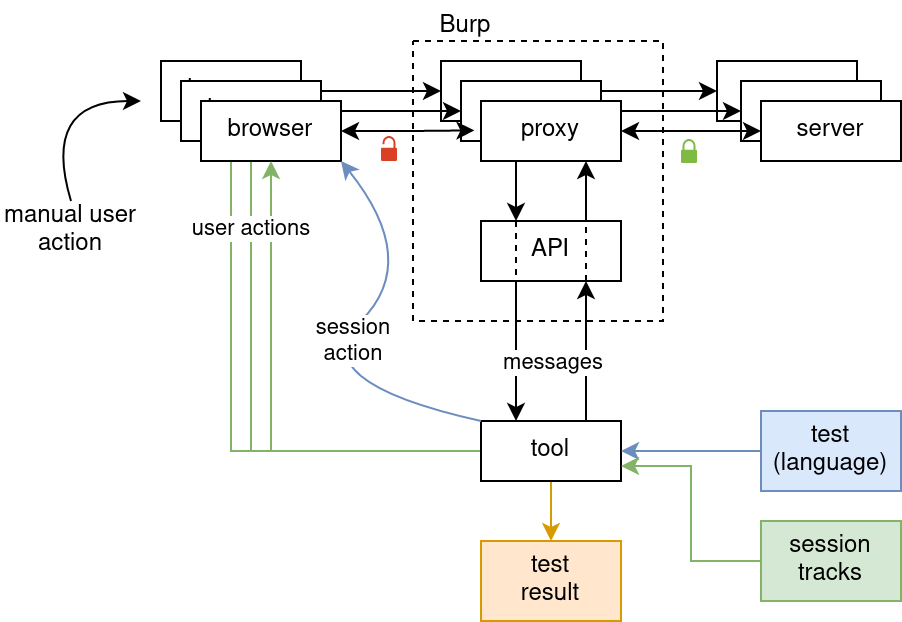
\includegraphics[width=\textwidth]{general_schema.png}
    \caption{General schema}
    \label{fig:general_schema}
\end{figure}

The components of the final tool can be seen in Figure \ref{fig:general_schema}. Burp Suite is composed of its proxy and related APIs; the tool will get all the messages from the proxy through the API, it will process them, and return them to the proxy. This way, all the messages will pass through the tool and make it possible to check and edit them.
Every browser, one for each session, will be using a dedicated proxy, which will act like a Man-In-The-Middle attack from the browser to the server, establishing a secure connection only on the last part of the communication to the server, making it possible to see plain HTTP communications on the browser side. Each browser will be supplied with the user actions taken from the session tracks specified beforehand. It is also possible to do manual user actions on the browser in case (for example) a captcha has to be resolved. Also, the session actions taken from the tests defined by the language can be supplied to the browser (for example, to pause or stop it). An essential component of the tool is the Test Suite defined with the language, which is supplied to the plugin, and executed with the sessions, eventually giving a result.

\section{The tool}
To implement the tool, I have decided to start from a work done by my colleague Wendy Barreto in her bachelor thesis \cite{wendy_barreto}, which realized a similar tool for \gls{OIDC} and \gls{OAuth} SSO protocols. This was a good base to start with the implementation. The interface of \cite{wendy_barreto} has been taken and adapted to fit the needs of this work. The tool code is written in Java, and the \Gls{burp}'s interface classes have been used to interact with it.
The standard usage of \Gls{burp} is based on the execution of a browser that connects to the \Gls{burp}'s proxy, in a way that all the packets can be intercepted, viewed or edited and forwarded or dropped from the \Gls{burp} interface. The tester would do some actions on the browser and watch the message flow in \Gls{burp} and then check them or edit them. With the tool, the idea is the same, but the operation is done on the browser, and the checks or edits on the messages are made automatically, in a way that the tester does not have to do them by itself.

\begin{figure}
    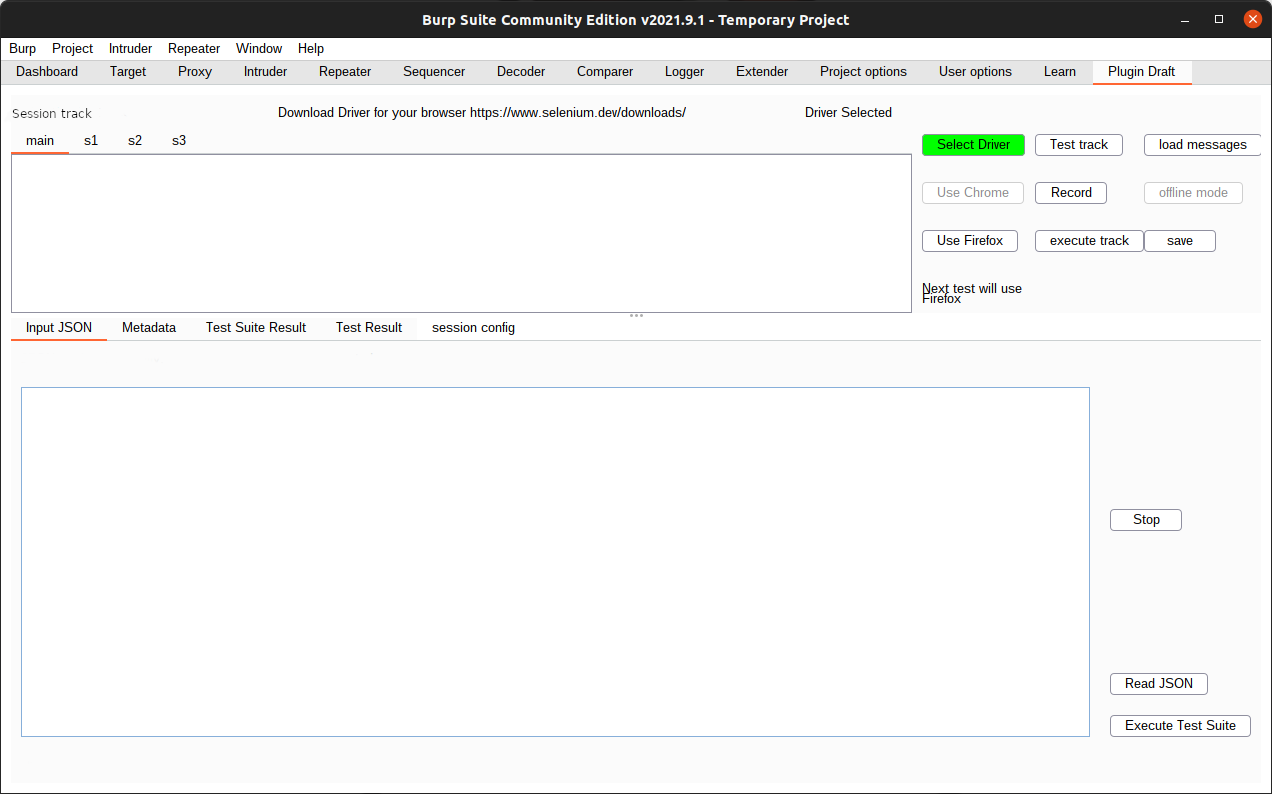
\includegraphics[width=\textwidth]{interface.png}
    \caption{Tool interface}
    \label{fig:plugin_interface}
\end{figure}

\subsection{User Interface of the tool}
In Figure \ref{fig:plugin_interface} the interface of the tool is shown. Starting from the top left, there is the session track input space, where a different track can be specified for each session. Following on the top right, a series of buttons that allow various configurations can be found:
\begin{itemize}
    \item \textbf{Use Chrome} or \textbf{Use Firefox} the browser to be used can be selected.
    \item \textbf{Select driver} the driver used to automate the actions on the browser can be selected.
    \item \textbf{Record} the record button can be used to record the flowing messages.
    \item \textbf{Load messages} the load messages button can be used to load the previously saved messages to be tested offline.
    \item \textbf{Offline mode} the offline mode button to test the loaded messages instead of the live ones.
    \item \textbf{Execute track} used to execute the session track without executing the tests, useful when the unaltered messages have to be saved.
    \item \textbf{Test track} used to test the session track without saving or doing any test.
\end{itemize}

In the bottom part, multiple tabs can be found:
\begin{itemize}
    \item \textbf{Input JSON} tab is used to load the tests written in the language into the tool, and with the use of two buttons, the language can be parsed, and the tests can be executed.
    \item \textbf{Test suite result} is the tab containing all the results of the executed tests.
    \item \textbf{Test result} is the tab used to see the specific test result, with all the intercepted messages related to it.
    \item \textbf{Session config} is used to configure the ports of the sessions that will be used in the tests.
\end{itemize}

In the bottom right part, when the \textbf{Input JSON} tab is selected, three buttons are available:
\begin{itemize}
    \item \textbf{Stop} used to stop the current execution.
    \item \textbf{Read JSON} used to read the written Tests.
    \item \textbf{Execute Test Suite} used to execute the written tests.
\end{itemize}

\subsection{Session managing}
The sessions are managed independently, and each session is basically a browser that is launched when a session is started. Each session can follow a different \gls{session track} defined in the apposite tabs. Every session is run in a separated thread to make parallelism between every session possible. Using specific commands in the language, it is possible to do some actions on each session, like stop it, pause it, or clear its cookies. Each browser uses a different proxy port so that it is possible to know from which session the messages come from, and so, being able to specific sessions in the tests.

\subsection{Test execution}
The test execution differs from passive to active, as passive tests do not need the edit of the messages, the execution of the \gls{session track} is done once the messages are saved, and the tests are executed on the saved messages. The possibility of exporting the saved messages to a file has also been added so that they can be imported into the tool and tested again.
On the other hand, active tests need to edit the messages, so the execution of the track has to be repeated for each test.

\subsection{Decoding \& encoding of parameters}
As said in Chapter \ref{chap:Design}, the decoding and encoding of parameters are possible. To do that, a list of encodings to be done on the parameter has to be provided, e.g., url, base64, deflate. Once the specified message is intercepted, the parameter is taken and decoded following the order of the provided encodings list. To do that, part of the code of SAML Raider \cite{saml_raider} has been used. SAML Raider is a \Gls{burp}'s plugin used to manage \Gls{SAML} certificates. The part of the code that deals with encoding and decoding the parameters has been taken and edited to fit the tool.

\subsection{SAML certificate managing}
In \Gls{SAML} Requests and responses, there is sometimes the need to remove or edit the certificate associated with that request or response, so, to speed up the process, a specific tag in the language has been added to remove or edit the certificate signature. There is still the possibility of doing the same removal by editing the \Gls{SAML} request or response with a regex, but with the use of the tag, this becomes more convenient.
To do this, a part of the code of SAML Raider \cite{saml_raider} has been used and edited to fit the needs of the tool.

\section{Problems and limitations encountered}
\label{sec:limitations}
During the implementation and the testing of the tool, multiple problems have been encountered, the majority of them have been solved, but some are still present. The most relevant ones will be discussed next:

\subsection{Automation problems}
One of the tool's limitations is the session track actions automation. Some captchas are often encountered during execution, making it impossible to proceed. Moreover, the track execution is limited, there is only a possible flow of actions (the one defined), and there is not the possibility of inserting ``if then else" constructs that could help to differentiate the actions based on the actual page or popup. For example, it could happen that a ``limited time offer" popup could appear in a website only in a particular time, the execution of the session track could be compromised by that, making impossible to distinguish whether the test failed because of the tested vulnerability or the actual popup.
Another problem in the automation part of the tool is that it is sometimes limited because the session track has to be defined over a specific website, doing a set of actions that are directly correlated to the website. Whenever the website is changed somehow, for example, the IDs or the button's position to be clicked change, the execution will fail because the track could not continue.
This is still not resolved, as no methods to make the track more dynamic have been found yet. This also means that every different web service that has to be tested will need a different session track to be defined, making it time-consuming to define. 

These Automation problems mainly occur when the service to be tested is not under the tester's control. Otherwise, captcha and popups could be easily deactivated for testing purposes. This means that this problem happens only in specific use case scenarios, so it is not a big deal.

\subsection{Oracle is sometimes ambiguous}
There is still a problem with the Oracle, where sometimes false positives or negatives arise if the tool's execution is interrupted for any reason. This is a problem because the interruption of the execution is a term of valuation for the Oracle. This means that the oracle will give a result also based on the correctness or incorrectness of the execution of the \gls{session track}. This makes it impossible to distinguish if the \gls{session track} has failed because of an error on the definition on it or because of an expected reason (like after a message modification).

\subsection{Interface and user feedbacks}
The tool's interface is a bit raw, and it is not very user-friendly. The user experience could be improved. I did not focus my attention on these topics during my work, but they are essential as the tool is not so easy to use. Also, the feedbacks of the errors encountered by the tool, such as execution errors or others, are not all shown to the user. This indeed has to be fixed, making more apparent to the end-user what is going wrong.






\clearpage
\chapter{Case Studies and Language Validation}
\label{chap:Use_cases}
%Una volta definito linguaggio e approccio abbiamo applicato il tool su due scenari e lia bbiamo potuti usare su due IDM protocols
% queste cose hanno portato ad avere queste due testsuites da poter usare..
Once the language and the approach to execute the tests have been defined and implemented, the tool has been applied to two different scenarios of IdM protocols, OAuth and SAML. In the end, two test suite has been defined, one for each protocol, that are ready to be used. This chapter will describe how this was done.

\section{OAuth \& OIDC Use-Case}    
To test the tool and the language during development, there was the need to specify a test suite to evaluate the correctness of their results. This was done starting from two works \cite{claudio_grisenti,wendy_barreto} that aimed at defining a set of tests to be done to test OAuth and OIDC protocols in a way that well-known vulnerabilities would be avoided. These two works have been chosen because the tests they present result from a deep examination. The \gls{OAuth} and \gls{OIDC} tests defined and used in \cite{claudio_grisenti,wendy_barreto} has then be re-defined in the language. Due to the newly available functionalities introduced with the language, new tests have been specified, especially active ones. In total, 7 active tests and 11 passive tests built the OAuth/OIDC test suite. These tests aim at testing the services against the well-known vulnerabilities to find out if the services are vulnerable. One of them can be found in Section \ref{sec:pkce_downgrade}. The complete list of tests with a brief description can be found in Table \ref{tab:OAuth_test_suite}.
%Dove l'abbiamo testato? quanti test attivi e quanti passivi? Cosa verificano? riportare un esempio magari? Citare che l'esempio del design c'è un test. Eseguito su un ambiente di test. Dove ho preso i test magari? è stato difficile tradurli? magari riportare un esecuzione del test (?). Tabella con tutti i test negli allegati o nella tesi. Esempio con un test magari. Spiego come ho tradotto i test.

\begin{table}[h]
    \begin{tabular}{|l|l|l|}
        \hline
        Test                                   & Type         & Description                             \\
        \hline\hline
        -CSRF protection (remove state)          & Active        & Tries to remove state parameter \\
        -CSRF protection (edit state)    &   Active  &   Tries to edit state parameter\\
        -PKCE Downgrade                  &   Active  &   Tries to remove code\_challenge parameter \\
        -PKCE plain supported            &   Active  &   Tries to remove code\_challenge\_method parameter \\
        -Redirect uri subdomain          &   Active  &   Tries to edit the redirect uri with subdomain \\
        -Redirect uri external domain    &   Active  &   Tries to edit the redirect uri with external domain \\
        State parameter replay          &   Active  &   Replay the parameter state from a session to another \\
        Parameter state is used         &   Passive  &   Check for the presence of the parameter state in \\
        -Compliance to Standard          &   Passive  &   Checks the presence of client\_id and response\_type\\
        -PKCE is implemented             &   Passive &   Check for common params presence \\
        PKCE method is not plain        &   Passive &   Check if param code\_challenge\_method=plain \\
        -Prevent clickjacking            &   Passive &   Check the headers values \\
        -Open redirectors: HTTP 307      &   Passive &   Check for 307 redirect \\
        -Block for Referrer header is used  &    Passive &   Checks for common parameters presence \\
        -Token saved as cookie in plain  &   Passive &   Check for the header cookie and search for token in it\\
        Client\_id is present            &   Passive &   Check for client\_id in all requests url \\
        Implicit grant not used         &   Passive &   Check for response\_type parameter \\ 
        Password credential\ grant not used  &   Passive &   Check for response\_type parameter \\

        \hline
    \end{tabular}
    \caption{\label{tab:OAuth_test_suite}OAuth/OIDC test suite}
\end{table}

\section{SAML Use-Case}
During the last stages of the development and testing of the tool, a strict collaboration between my colleague Sofia Zanrosso and me has started. Her objective was to create a \gls{SAML} Test Suite to facilitate automatic penetration testing over \gls{SAML} \cite{sofia_zanrosso}. The tool defined in this thesis was compared with other ones and was used to define and execute the tests. During the progress of both our works, a lot of feedback and bugs have been reported to me, speeding up the testing phase of the tool. At the same time, we found that my tool was in some respects better compared to the other alternatives. For example:
\begin{itemize}
    \item Other plugins were giving false positives on some tests
    \item ``the previously employed transition times between tools have been greatly reduced"
    \item ``making it possible to analyze almost completely the vulnerabilities of the tested subjects"
\end{itemize}
In the end, it has been possible to define all the necessary tests and to execute them to test the services.

\section{Expirience during the use of the language}
Experience during the use of the language.
Many tests have been translated or defined into the language during the two preceding case studies. This has not been difficult to do. In total, 18 tests for OAuth and 86 tests for SAML have been defined. The process of defining or translating a test involves the identification of the messages to be intercepted, the actions to be done on them, how many sessions are needed, and the parts of the messages to be checked to give a result of the test. Once these four main components have been identified, the next step is to declare everything from the Message Type to the checks. The most difficult part is probably the definition of a Message Type to intercept a message, as it is sometimes difficult to filter the messages.






\clearpage
\chapter{Related works}
\label{chap:Related_work}
This chapter will describe software and tools related to the work in this thesis.

\section{Micro-Id-Gym}
\label{sec:micro-id-gym}
Micro ID Gym (MIG) ``aims to assist system administrators and testers in the deployment and pen-testing of IdM protocol instances" - \cite{micro_id_gym}, inside this tool, two pentesting tools can be found:
\begin{itemize}
    \item MIG - OAuth/OIDC \cite{claudio_grisenti}
    \item MIG - SAML SSO \cite{stefano_facchini}
\end{itemize}
They are both plugins for \Gls{burp}, which have as objective to test the two different protocols. These plugins execute a series of actions on a browser, check the messages in the background, and then provide a result.
These two plugins are related to mine, but they are specifically created and defined to test SSO protocols only, and the tests they used are fixed and cannot be easily edited. If a new test has to be implemented, the plugin must be recompiled.

\section{SSO Testing language and Plugin}
The preceding two tools of MIG found in Section \ref{sec:micro-id-gym} have been improved by the work done by my colleague Wendy Barreto \cite{wendy_barreto} in her bachelor thesis at Università di Trento to test \gls{OAuth} and \gls{OIDC} SSO protocols with a custom test definition pattern. Her work aimed to fix the problem of hard-coded tests in the plugins for SSO protocols testing. The previous MIG plugin had been improved by removing the staticity of the test, adding the possibility to define all the tests with the use of a JSON language.
The available test actions worked well, but there were some limitations on the possible actions, especially in active tests. For example:
\begin{itemize}
    \item Limited oracle for the verification of active tests, having just the verification of the correct execution of the operation and a check for the string ``error" on the last page of the browser
    \item The filtering of the message to check or edit for static tests is limited, only \textit{Authorization grant message}, \textit{Response messages}, \textit{Request messages} and \textit{All messages} are available
    \item Only regex are supported to search what is needed in a message
    \item Impossibility to work over encoded parameters
    \item Impossibility of doing multiple operations on a single message
    \item Impossibility of saving a parameter and using it somewhere else
    \item Impossibility of using multiple sessions in a test
\end{itemize}
Some of these limitations were stated as future works in \cite{wendy_barreto}. A complete list of differences between the two languages and tools can be found in Attachment \ref{attachment:languages_comparison}.

Previously in this thesis, it has been said that part of this work has been taken as a base to start with the implementation of the tool. The idea of a language that could be used for any test over browser-based protocols was born when I used her plugin, which was limited to \gls{OAuth} and \gls{OIDC} tests. I wanted to enlarge the possible tests to be defined without a restriction on a specific protocol. 
One of the things that have been used is the interface of the plugin, which has been modified, adding buttons and tabs to deal with multiple \gls{session track}s and other added functionalities. Also, the automation of the \gls{session track} was taken and edited. This part was already used in \cite{claudio_grisenti,stefano_facchini}.




\clearpage
\chapter{Conclusions, Limitations and Future Works}
One of the biggest limitations that the tool has is the session track actions automations, it often happens that some captcha are encountered during execution, making impossible to proceed. Moreover, the track execution is limited, there is only a possible flow of actions (the one defined) and there is not the possibility of inserting if then else constructs that could help to differentiate the actions based on the actual page or popup. For example, it could happen that an "limited time offer" popup could appear in a website only in a particular time, the execution of the session track could be compromised by that, making impossible to distinguish wether the test failed because of the tested vulnerability or the actual popup.






\endgroup 
% bibliografia in formato bibtex
%
% aggiunta del capitolo nell'indice
\addcontentsline{toc}{chapter}{Bibliografia}
% stile con ordinamento alfabetico in funzione degli autori
\bibliographystyle{plain}
\bibliography{biblio}
%%%%%%%%%%%%%%%%%%%%%%%%%%%%%%%%%%%%%%%%%%%%%%%%%%%%%%%%%%%%%%%%%%%%%%%%%%
%%%%%%%%%%%%%%%%%%%%%%%%%%%%%%%%%%%%%%%%%%%%%%%%%%%%%%%%%%%%%%%%%%%%%%%%%%
%% Nota
%%%%%%%%%%%%%%%%%%%%%%%%%%%%%%%%%%%%%%%%%%%%%%%%%%%%%%%%%%%%%%%%%%%%%%%%%%
%% Nella bibliografia devono essere riportati tutte le fonti consultate 
%% per lo svolgimento della tesi. La bibliografia deve essere redatta 
%% in ordine alfabetico sul cognome del primo autore. 
%% 
%% La forma della citazione bibliografica va inserita secondo la fonte utilizzata:
%% 
%% LIBRI
%% Cognome e iniziale del nome autore/autori, la data di edizione, titolo, casa editrice, eventuale numero dell’edizione. 
%% 
%% ARTICOLI DI RIVISTA
%% Cognome e iniziale del nome autore/autori, titolo articolo, titolo rivista, volume, numero, numero di pagine.
%% 
%% ARTICOLI DI CONFERENZA
%% Cognome e iniziale del nome autore/autori (anno), titolo articolo, titolo conferenza, luogo della conferenza (città e paese), date della conferenza, numero di pagine. 
%% 
%% SITOGRAFIA
%% La sitografia contiene un elenco di indirizzi Web consultati e disposti in ordine alfabetico. 
%% E’ necessario:
%%   Copiare la URL (l’indirizzo web) specifica della pagina consultata
%%   Se disponibile, indicare il cognome e nome dell’autore, il titolo ed eventuale sottotitolo del testo
%%   Se disponibile, inserire la data di ultima consultazione della risorsa (gg/mm/aaaa).    
%%%%%%%%%%%%%%%%%%%%%%%%%%%%%%%%%%%%%%%%%%%%%%%%%%%%%%%%%%%%%%%%%%%%%%%%%%
%%%%%%%%%%%%%%%%%%%%%%%%%%%%%%%%%%%%%%%%%%%%%%%%%%%%%%%%%%%%%%%%%%%%%%%%%%

\titleformat{\chapter}
{\normalfont\Huge\bfseries}{Attachment \thechapter}{1em}{}
% sezione Allegati - opzionale
\appendix
\chapter{PKCE test Example complete}
\label{chap:PKCE_complete}
\begin{lstlisting}[language=json]
{
    "test suite": {
        "name": "OAuth Active tests",
        "description": "A series of tests to test OAuth's well-known vulnerabilities",
        "filter messages": true
    },
    "tests": [     
        {
            "test": {
                "name": "PKCE Downgrade",
                "description": "Tries to remove code_challenge parameter",
                "type": "active",
                "sessions": [
                    "s1"
                ],
                "operations": [
                    {
                        "session": "s1",
                        "action": "start"
                    },
                    {
                        "action": "intercept",
                        "from session": "s1",
                        "then": "forward",
                        "message type": "authorization request",
                        "preconditions": [
                            {
                                "in": "url",
                                "check param": "code_challenge",
                                "is present": true
                            }
                        ],
                        "message operations": [
                            {
                                "from": "url",
                                "remove parameter": "code_challenge"
                            }
                        ]
                    }
                ],
                "result": "incorrect flow s1"
            }
        }
    ]
}
\end{lstlisting}

\chapter{Language comparison}
\label{attachment:languages_comparison}

\begin{center}
    \begin{tabular}{ |c|c|c| }
        \hline
        Action                                    & Old language         & New language                             \\
        \hline\hline
        Custom message filtering                  & Only on active tests & supported                                \\
        Edit string                               & only by regex        & supported with regex and check construct \\
        Remove string                             & only by regex        & supported with regex and check construct \\
        Add string                                & not supported        & supported                                \\
        Check parameter                           & only with regex      & with regex and check construct           \\
        Multiple operations in single message     & not supported        & supported                                \\
        Saving and reusing of values and messages & not supported        & supported                                \\
        Multiple sessions in single test          & not supported        & supported                                \\
        Custom oracle definition                  & not supported        & by using regex and checks                \\
        \hline
    \end{tabular}
\end{center}






\end{document}
